\def\year{2021}\relax
%File: formatting-instructions-latex-2021.tex
%release 2021.2
\documentclass[letterpaper]{article} % DO NOT CHANGE THIS
\usepackage{aaai21}  % DO NOT CHANGE THIS
\usepackage{times,xcolor,booktabs,tabularx}  % DO NOT CHANGE THIS
\usepackage{helvet} % DO NOT CHANGE THIS
\usepackage{courier}  % DO NOT CHANGE THIS
\usepackage[hyphens]{url}  % DO NOT CHANGE THIS
\usepackage{graphicx} % DO NOT CHANGE THIS
\urlstyle{rm} % DO NOT CHANGE THIS
\def\UrlFont{\rm}  % DO NOT CHANGE THIS
\usepackage{natbib}  % DO NOT CHANGE THIS AND DO NOT ADD ANY OPTIONS TO IT

\usepackage{caption} % DO NOT CHANGE THIS AND DO NOT ADD ANY OPTIONS TO IT
\frenchspacing  % DO NOT CHANGE THIS
\setlength{\pdfpagewidth}{8.5in}  % DO NOT CHANGE THIS
\setlength{\pdfpageheight}{11in}  % DO NOT CHANGE THIS
%\nocopyright
%PDF Info Is REQUIRED.
% For /Author, add all authors within the parentheses, separated by commas. No accents or commands.
% For /Title, add Title in Mixed Case. No accents or commands. Retain the parentheses.
\pdfinfo{
	/Title (AAAI Press Formatting Instructions for Authors Using LaTeX -- A Guide)
	/Author (AAAI Press Staff, Pater Patel Schneider, Sunil Issar, J. Scott Penberthy, George Ferguson, Hans Guesgen, Francisco Cruz, Marc Pujol-Gonzalez)
	/TemplateVersion (2021.2)
} %Leave this
% /Title ()
% Put your actual complete title (no codes, scripts, shortcuts, or LaTeX commands) within the parentheses in mixed case
% Leave the space between \Title and the beginning parenthesis alone
% /Author ()
% Put your actual complete list of authors (no codes, scripts, shortcuts, or LaTeX commands) within the parentheses in mixed case.
% Each author should be only by a comma. If the name contains accents, remove them. If there are any LaTeX commands,
% remove them.

% DISALLOWED PACKAGES
% \usepackage{authblk} -- This package is specifically forbidden
% \usepackage{balance} -- This package is specifically forbidden
% \usepackage{color (if used in text)
% \usepackage{CJK} -- This package is specifically forbidden
% \usepackage{float} -- This package is specifically forbidden
% \usepackage{flushend} -- This package is specifically forbidden
% \usepackage{fontenc} -- This package is specifically forbidden
% \usepackage{fullpage} -- This package is specifically forbidden
% \usepackage{geometry} -- This package is specifically forbidden
% \usepackage{grffile} -- This package is specifically forbidden
% \usepackage{hyperref} -- This package is specifically forbidden
% \usepackage{navigator} -- This package is specifically forbidden
% (or any other package that embeds links such as navigator or hyperref)
% \indentfirst} -- This package is specifically forbidden
% \layout} -- This package is specifically forbidden
% \multicol} -- This package is specifically forbidden
% \nameref} -- This package is specifically forbidden
% \usepackage{savetrees} -- This package is specifically forbidden
% \usepackage{setspace} -- This package is specifically forbidden
% \usepackage{stfloats} -- This package is specifically forbidden
% \usepackage{tabu} -- This package is specifically forbidden
% \usepackage{titlesec} -- This package is specifically forbidden
% \usepackage{tocbibind} -- This package is specifically forbidden
% \usepackage{ulem} -- This package is specifically forbidden
% \usepackage{wrapfig} -- This package is specifically forbidden
% DISALLOWED COMMANDS
% \nocopyright -- Your paper will not be published if you use this command
% \addtolength -- This command may not be used
% \balance -- This command may not be used
% \baselinestretch -- Your paper will not be published if you use this command
% \clearpage -- No page breaks of any kind may be used for the final version of your paper
% \columnsep -- This command may not be used
% \newpage -- No page breaks of any kind may be used for the final version of your paper
% \pagebreak -- No page breaks of any kind may be used for the final version of your paperr
% \pagestyle -- This command may not be used
% \tiny -- This is not an acceptable font size.
% \vspace{- -- No negative value may be used in proximity of a caption, figure, table, section, subsection, subsubsection, or reference
% \vskip{- -- No negative value may be used to alter spacing above or below a caption, figure, table, section, subsection, subsubsection, or reference

\setcounter{secnumdepth}{0} %May be changed to 1 or 2 if section numbers are desired.

% The file aaai21.sty is the style file for AAAI Press
% proceedings, working notes, and technical reports.
%

% Title

% Your title must be in mixed case, not sentence case.
% That means all verbs (including short verbs like be, is, using,and go),
% nouns, adverbs, adjectives should be capitalized, including both words in hyphenated terms, while
% articles, conjunctions, and prepositions are lower case unless they
% directly follow a colon or long dash

\title{Risk and Survival Analysis from COVID Outbreak Data : Lessons from India}
\author{
	Prasad Bankar\textsuperscript{\rm *}, Subhasis Panda\textsuperscript{\rm *}, Vaibhav Anand\textsuperscript{\rm *},  Vineet Kumar\footnote{Equal Contribution, Names appear in alphabetical order.}
	% All authors must be in the same font size and format.
	\\
}
\affiliations{
	%Afiliations
	Indian Institute of Technology\\
	Kharagpur, WB, India, 721302 \\
	%If you have multiple authors and multiple affiliations
	% use superscripts in text and roman font to identify them.
	%For example,
	
	% Sunil Issar, \textsuperscript{\rm 2}
	% J. Scott Penberthy, \textsuperscript{\rm 3}
	% George Ferguson,\textsuperscript{\rm 4}
	% Hans Guesgen, \textsuperscript{\rm 5}.
	% Note that the comma should be placed BEFORE the superscript for optimum readability
	
	%    \textsuperscript{\rm 2}Indian Statistical Institute\\
	%    Kolkata, WB, India, 700108\\
	% email address must be in roman text type, not monospace or sans serif
	
	
	\{prasadbankar33,subhasispanda94,vaibhav.hk.anand,vntkumar8\}gmail.com
	% See more examples next
}
\iffalse
%Example, Single Author, ->> remove \iffalse,\fi and place them surrounding AAAI title to use it
\title{My Publication Title --- Single Author}
\author {
	% Author
	Author Name \\
}

\affiliations{
	Affiliation \\
	Affiliation Line 2 \\
	name@example.com
}
\fi

\iffalse
%Example, Multiple Authors, ->> remove \iffalse,\fi and place them surrounding AAAI title to use it
\title{My Publication Title --- Multiple Authors}
\author {
	% Authors
	First Author Name,\textsuperscript{\rm 1}
	Second Author Name, \textsuperscript{\rm 2}
	Third Author Name \textsuperscript{\rm 1} \\
}
\affiliations {
	% Affiliations
	\textsuperscript{\rm 1} Affiliation 1 \\
	\textsuperscript{\rm 2} Affiliation 2 \\
	firstAuthor@affiliation1.com, secondAuthor@affilation2.com, thirdAuthor@affiliation1.com
}
\fi
\begin{document}
	
	\maketitle
	
	\begin{abstract}
		
		The present analysis is an attempt to provide data-backed evidence around mortality due to COVID-19 in Indian context. We provide a description of the prevailing COVID-19 conditions in India by means of succinct visualisation via a dynamic dashboard and cluster analysis. Building upon this, we performed survival analysis on COVID-19 patients from the state of Karnataka, stratifying the data on the basis of age and gender. The findings of the same have been reported in this paper. To our knowledge, this is the largest retrospective cohort-based survival analysis in Indian context.
	\end{abstract}
	\section{Introduction}
	\noindent The Novel Coronavirus is spreading fast. While India is attempting to unlock the economy fully, the number of new cases per day is still 40,000. Actionable insights to contain the spread is the need of the hour.
	Modelling and Forecasting COVID-19 is very difficult given the unreasonable modelling assumption, lack of good quality data \cite{ioannidis2020forecasting}. 
	
	
	\begin{figure}[h]
		\centering
		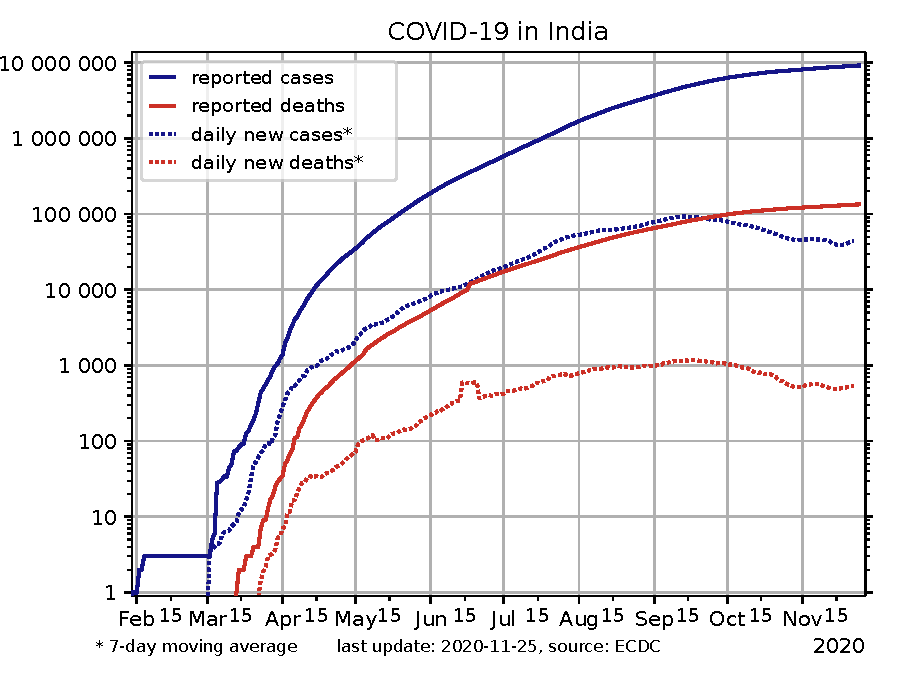
\includegraphics[width=0.95\linewidth]{log-case}
		\caption{Daily COVID-19 cases in India (Log Scale)}
		\label{fig:india-log}
	\end{figure}
	
	Keeping this goal in mind, we developed a dashboard to enable policymakers to extract a variety of information from publicly available data on COVID-19. The dashboard provides risk summaries and enables users to look at data from different perspectives, arriving at actionable insights. The COVID–19 situation may be described through a number of characteristics such as the rate of occurrence of new cases, the breakup of confirmed cases by severity, rate of recovery, number of active cases, rate of testing, rate of detection of new cases through tests, and death rate. 
	
	When measured and presented appropriately, each of these characteristics communicates a different aspect of the overall scenario. Sometimes, a combination of a few characteristics may also be used. These characteristics or their combinations are called dimensions. We attempted to cover all the dimensions and a few others not described above. We also included some composite dimensions obtained by combining values of two or more directly observed dimensions. Although we intended to cover many dimensions, a few like the breakup of confirmed cases by severity could not be covered as data were not available. We observed that the daily recovery varies widely and is low in many states and cities. Daily recovery is even zero on several occasions and frequently varies by over five times or more on subsequent days. The process of recovery comprises of interdependent activities like sample collection, testing, retesting, and approval of final release. It is well-known that built-in delays in such processes are often over 50\% of the total time and standard techniques exist to reduce the cycle time drastically.
	
	We also used survival analysis to compute the infection fatality rate (IFR) in the two critical states of India, viz. Tamil Nadu and Karnataka. We did a cohort selection with age and gender as variates separately. Using Kaplan-Meier estimate and Log Rank Test, we tried to model the recovery and fatality rate. We tried to analyse the effect of co-morbidity on the COVID-19 fatality rate. We performed a cluster analysis with the different districts of Karnataka to understand the disease spread.
	
	The paper is organized as follows --- first, we describe our approach for understanding the holistic picture of COVID-19 spread, testing and risk in India. We performed the elementary descriptive analysis. We also provide the case based clustering of Indian states. Subsequently, we performed survival analysis by building our cohort of patients. 
	\section{Covid Risk Analysis}\label{dash}
	When COVID-19 struck, the governments across the globe started enforcing the policy of lockdown. The Government of India followed suit and a strict lockdown was imposed on 25th March, 2020. However, the lockdown was just a measure to reduce the speed and extent of the spread of COVID-19. Recognising that the policymakers could benefit from a tool that facilitated visualisation along different dimensions, we built an interactive dashboard, using real-time data, via the Panel library in Python. We are thankful to \citet{covid19indiaorg2020tracker} for providing the public api for the data. The dashboard \footnote{https://covid-isical.tech/} aimed at supporting the ``unlock'' strategy design and facilitate intervention monitoring. It provided the following functionalities:
	\begin{itemize}
		\item Macro-level view: The dashboard allows the policymakers to have a birds-eye view of the country as well as individual States. This was achieved by means of a risk summary table and geographical heat-maps.
		\item Spread Assessment Metrics:
		\begin{itemize}
			\item Average confirmed cases / day: Increasing trend of occurrence of new cases is likely to indicate that the virus is spreading.
			\item Active cases: Increasing trend of active cases indicates the possibility of increased stress on resources at present or in the near future.
		\end{itemize}
		\item Risk Assessment Metrics:
		\begin{itemize}
			\item Avg. Confirmed Cases to Avg. Recoveries in Consecutive Weeks Traffic Intensity (a term from queuing theory): It acted as a leading indicator of stress on resources, with values $>$ 1  implying faster arrival of new cases compared to recovery.
			\begin{figure}[h!]
				\centering
				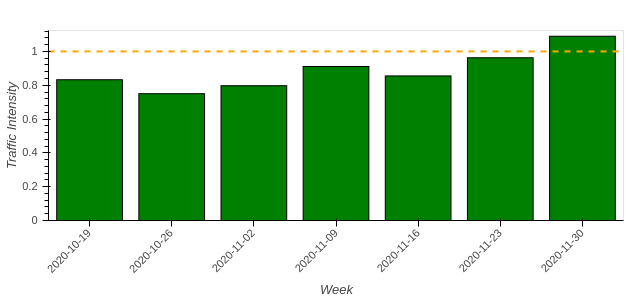
\includegraphics[width=\linewidth]{ti}
				\caption{Traffic Intensity across last 7 weeks}
				\label{fig:ti}
			\end{figure}
			
			\item Points plot of Tests in Each Week and \% Positive in each week: Higher proportion positive  test results on a larger test population (possibly less targeting) are anomalous and need investigation. There are at least three possibilities: 
			\begin{quote}
				\begin{enumerate}
					\item A rapid increase in the rate of infection 
					\item Carrying out tests in new (hitherto untested) areas with a high but unknown rate of infection 
					\item Improper testing leading to many incorrectly positive results
					
				\end{enumerate}
			\end{quote}
			\begin{figure}[h!]
				\centering
				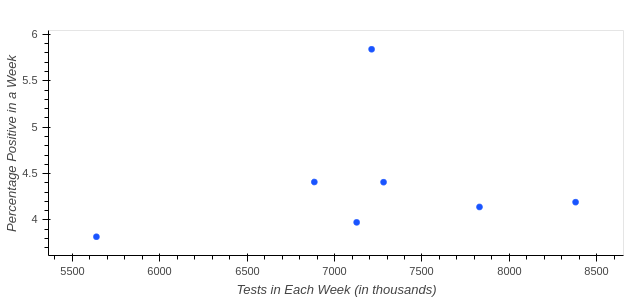
\includegraphics[width=1\linewidth]{pp}
				\caption{Assessing adequacy of testing in India}
				\label{fig:pp}
			\end{figure}
			
		\end{itemize}
	\end{itemize}
	We also provided a tool for the comparative assessment of Indian states using colour-coded heatmaps showing the top States in India w.r.t confirmed, recovered, and deceased cases, respectively. 
	
	\subsection{Cluster Analysis} In any nation, when a COVID-19 outbreak occurred. there were some states/provinces/regions which were more affected as compared to other states/provinces/regions. The motivation behind performing cluster analysis is identifying such underlying structures within the COVID-19 cases. We performed euclidean measure based vanilla k-means clustering on the top 20 most affected states. We chose the value of k by iteratively experimenting and checking the standard silhouette score and elbow metric.
	\begin{figure}[h!]
		\centering
		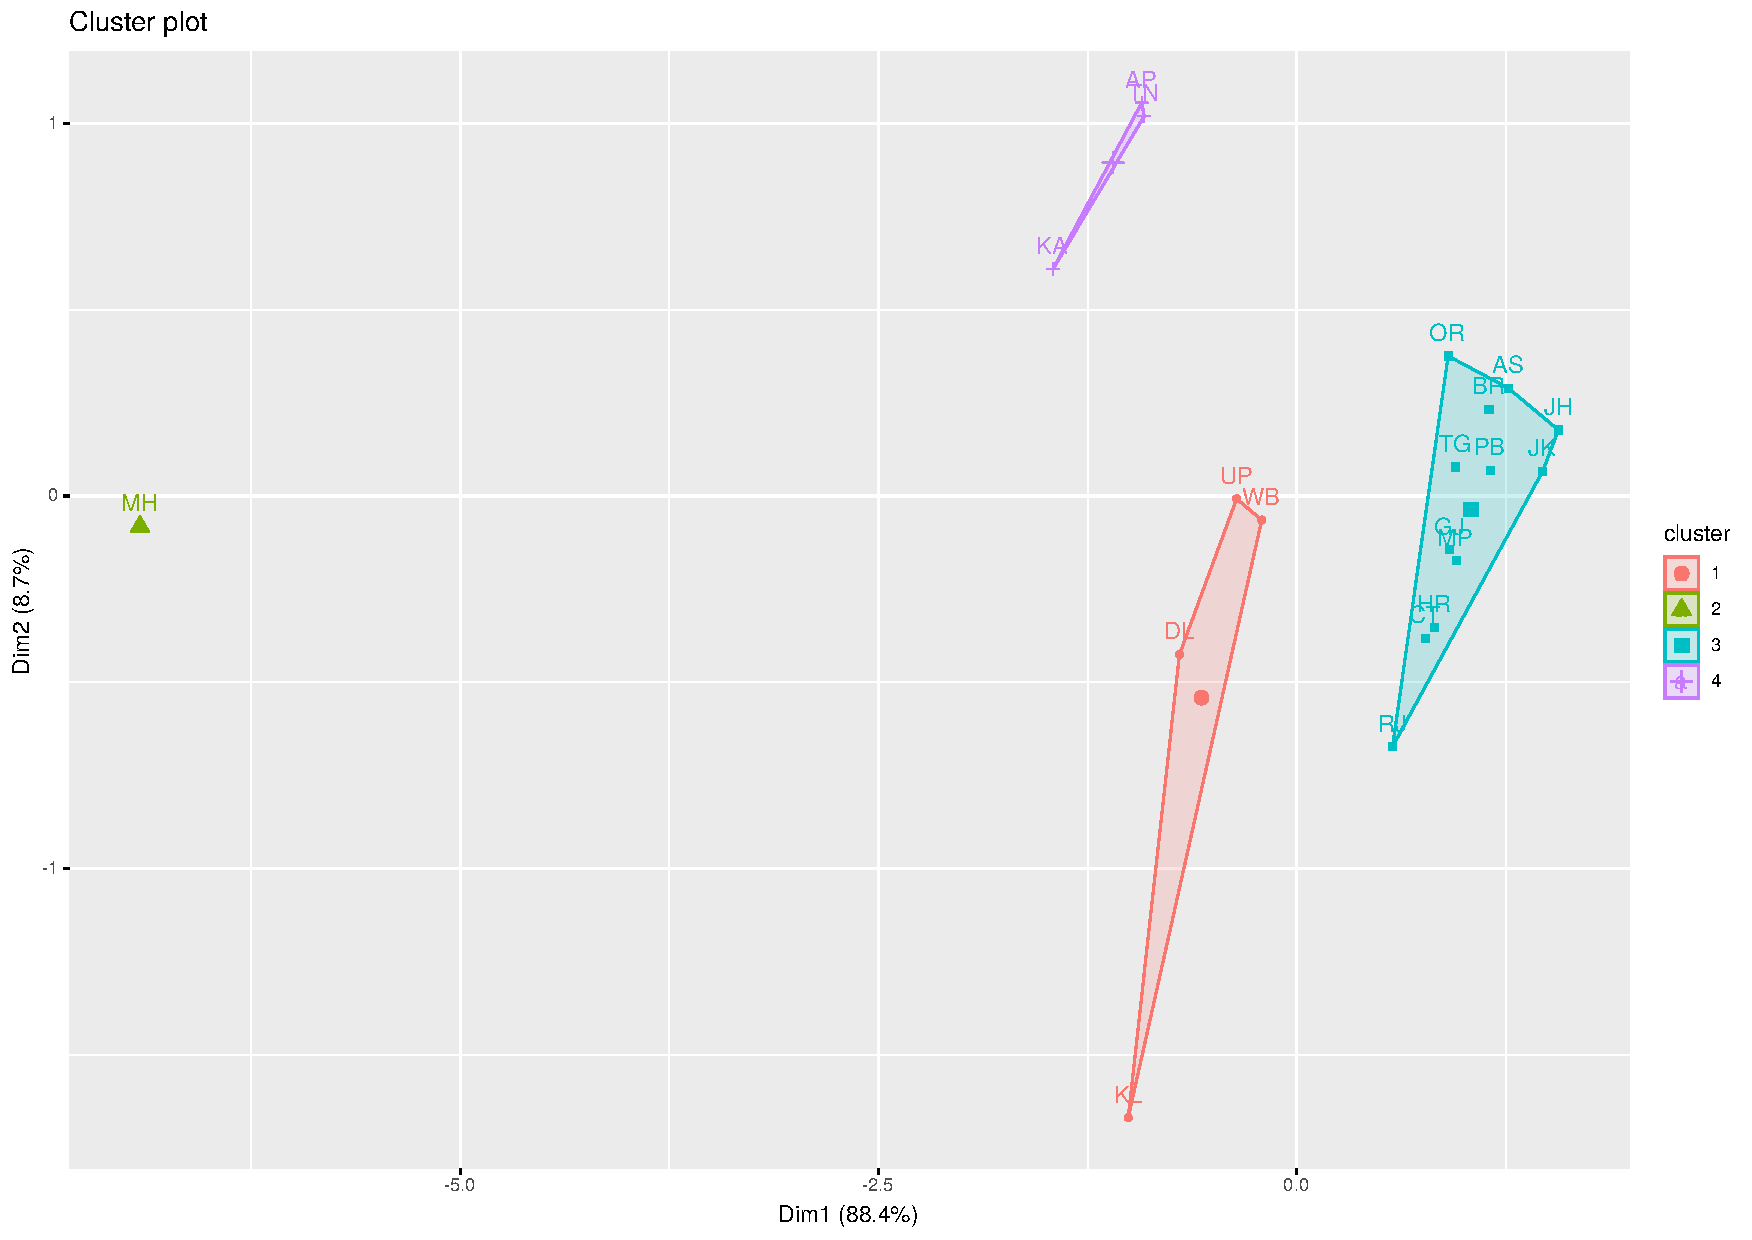
\includegraphics[width=\linewidth]{cluster}
		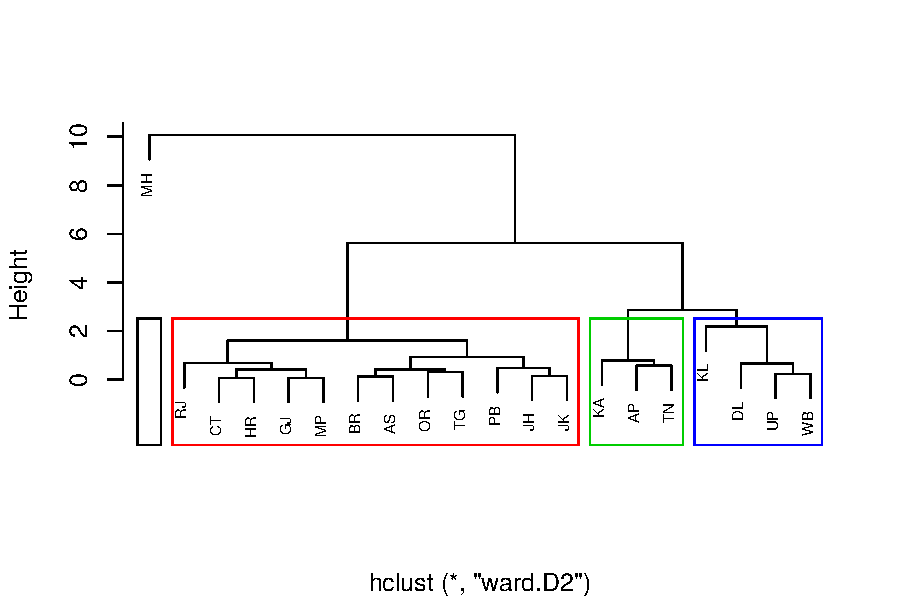
\includegraphics[width=\linewidth]{hc}
		\caption{Clustering analysis (K-means and AGNES)}
		\label{fig:cluster}
	\end{figure}
	We also performed  the hierarchical clustering on the cases using Ward distance (chosen among other competing metric based on Agglomerative coefficient). Structures thus formed have physical meaning and interpretation. For instance, MH is the worst affected state, while \{KL, DL, UP, WB\} are among the second worst-hit states. Such clustering analysis, performed across the last 7-8 months, could give a better picture of how a less affected state shifts from one cluster to another as cases increase and vice-versa. 
	
	\section{Covid Survival Analysis}\label{surv}
	
	
	In this section, we will discuss our approach of performing survival analysis \cite{pocock2002survival} on the COVID-19 cases of India.  There has been minimal work on COVID-19 survival analysis data. One such work in the Indian context has been done by \citet{mishra2020covid}. However, their cohort size is very limited, with $<$ 500 patients. Hence, findings are  not very conclusive owing to the small sample size. 	In the present study, we illustrate survival analysis results on a reasonably large cohort of patients (26,714 patients) from the Indian State of Karnataka.
	
	
	
	
	\subsection{Dataset Description \& Methods}
	
	Using the data of testing date and the date of discharge (either due to recovery or death) from  hospitals for individual patients in Karnataka, the probabilities of a person being in infected condition as the days progress are calculated using Kaplan-Meier estimator of the survival function. Our particular work aims to study the difference in recovery time among gender and various age groups. 
	\paragraph{Cohort Selection}
	
	
	We downloaded the patient-specific data containing patient id, age, gender,  admit date and cure/deceased date from \citet{AGM-2020}. These data were sourced from official government medical bulletins and recorded neatly into a spreadsheet. 
	We calculated the number of days to recovery/death for each patient by subtracting the admit date with the discharge date.  
	
	
	We selected all such patients who were admitted in Karnataka as reported by government bulletins. We excluded four patients --- one patient was a transgender, one patient had unusually high recovery time (84 days), and two patients did not have gender information. We selected only such patients who had a definite outcome -- either recovered or deceased. We excluded the active cases. Our final cohort size was 26,741 patients. Age distribution of patients is shown in Fig: \ref{fig:age}. 
	
	\begin{figure}[h]
		\centering
		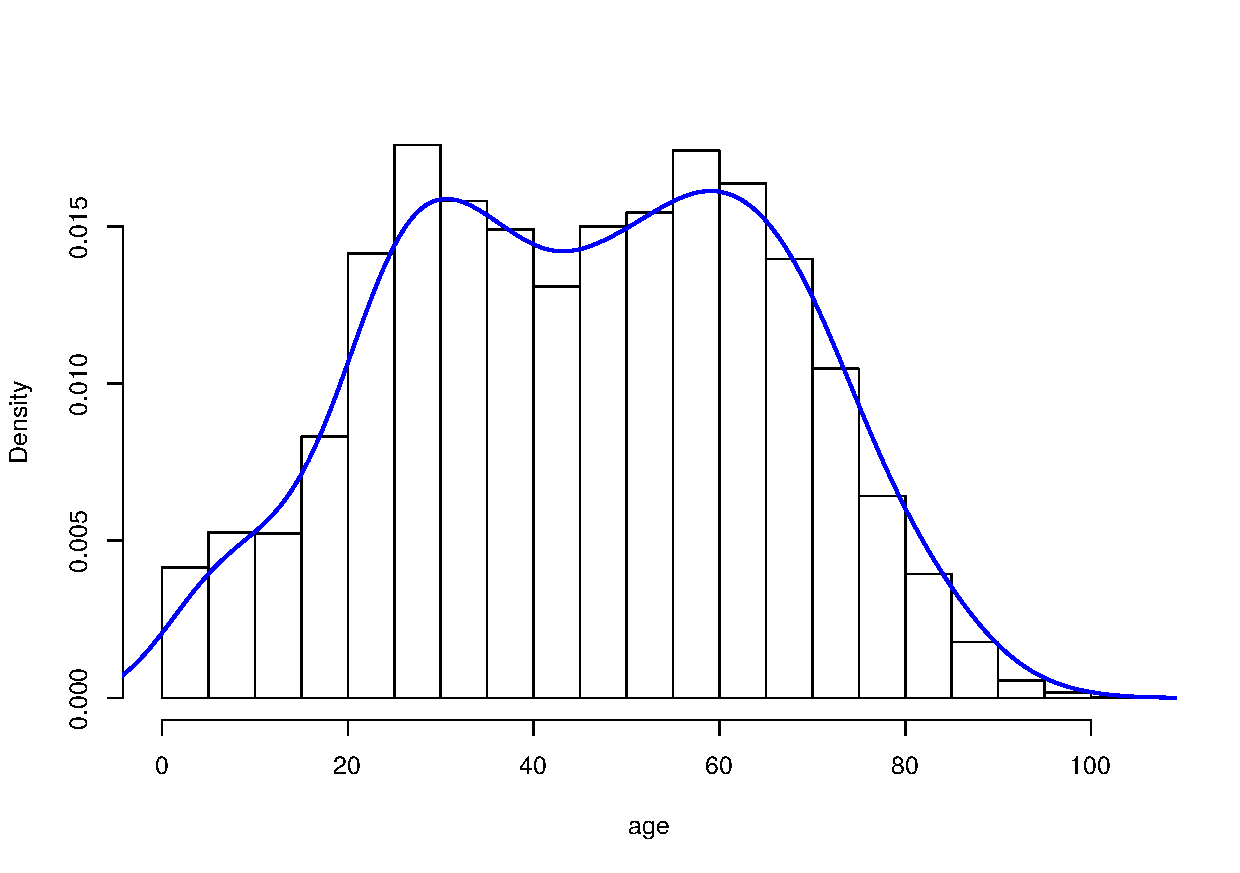
\includegraphics[width=0.9\linewidth]{age}
		\caption{{Age} \normalcolor distribution of patients}
		\label{fig:age}
	\end{figure}
	
	In our selected cohort, the mean age is 37 years (median 36) and the mean time to recovery is 8 days. Similarly, the stay distribution is shown in Fig: \ref{fig:stay}. 
	
	
	\begin{figure}[h]
		\centering
		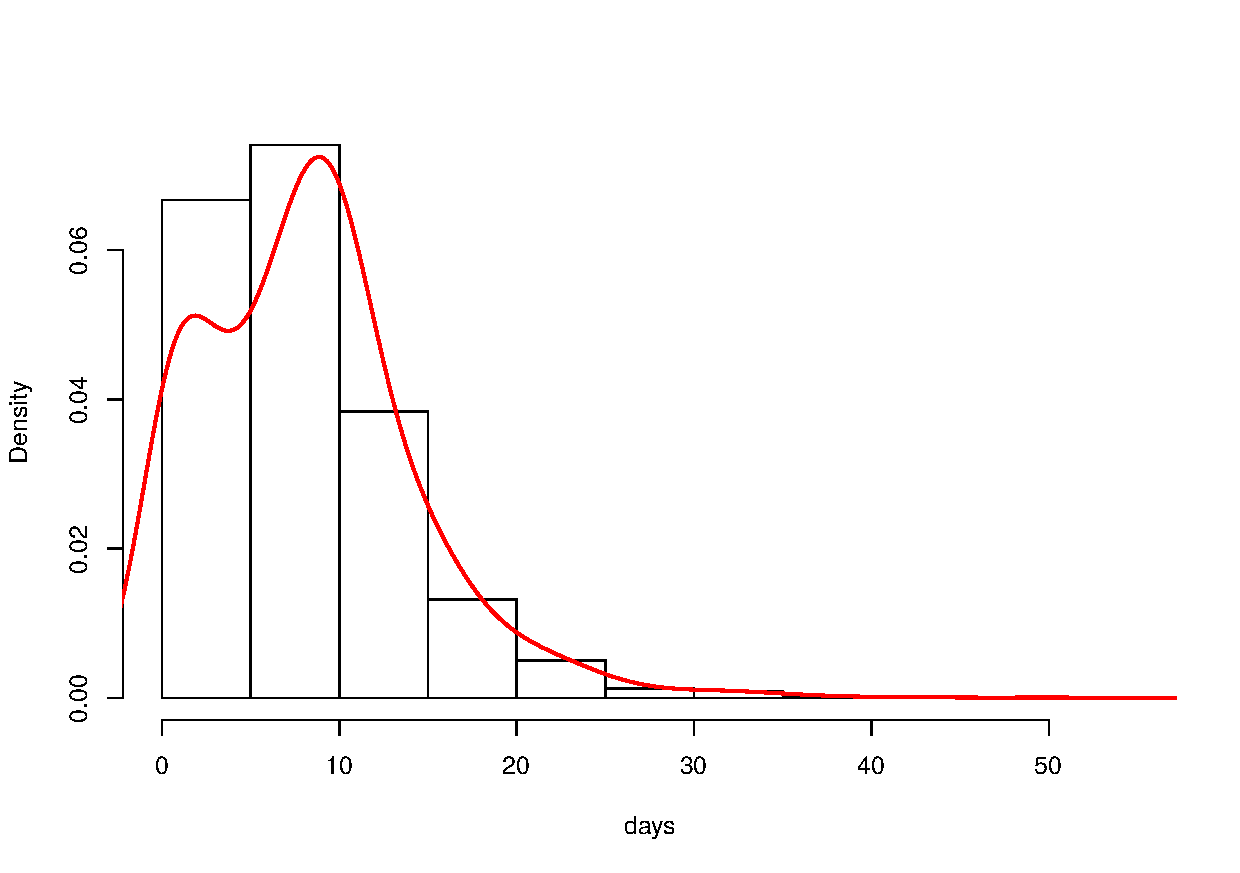
\includegraphics[width=0.9\linewidth]{stay}
		\caption{ {Stay} \normalcolor distribution of patients}
		\label{fig:stay}
	\end{figure}
	
	%\textbf{Median survival days} for \underline{Male and Female is 14 and 21 days} respectively. 
	\begin{table*}[h!]
		\centering
		\begin{tabular}{@{}lccc@{}}
			\toprule
			& Infected & Recovered & Median Survival Time (days) \\ \midrule
			\textbf{Total infected}                                & 26741    & 15231     & 10 (8-13)            \\
			Male                                                   & 17451    & 9472      & 10 (8-13)            \\
			Female                                                 & 9290     & 5759      & 10 (8-13)            \\\midrule
			\textbf{Total infected age  $\leq$ 18}             & 2295     & 2258      & 10 (8-14)            \\
			Total infected age $\leq$ 18 Male                 & 1223     & 1200      & 10 (8-14)            \\
			Total infected age $\leq$ 18 Female               & 1072     & 1058      & 10 (8-14)            \\\midrule
			\textbf{Total infected 18\textless{}age \textless{}60} & 16380    & 11809     & 10 (8-13)            \\
			Total infected 18\textless{}age \textless{}60 Male     & 10715    & 7574      & 10 (8-13)            \\
			Total infected 18\textless{}age \textless{}60 Female   & 5665     & 4235      & 10 (8-13)            \\\midrule
			\textbf{Total infected age  $\geq$ 60}          & 8066     & 1164      & 10 (8-13)            \\
			Total infected age $\geq$ 60 Male              & 5513     & 698       & 10 (8-13)            \\
			Total infected age $\geq$ 60 Female            & 2553     & 466       & 10 (8-13)            \\ \bottomrule
			
			\label{t1}
		\end{tabular}
		\caption{ Median recovery time of infected population}
		\label{table:t1}
	\end{table*}
	
	\subsection{Gender Stratified KM Estimate}
	To perform the Kaplan-Meier survival estimate \cite{kaplan1958nonparametric}, we stratified our cohort gender-wise -- male and female. 
	The estimator of the survival function ${\displaystyle S(t)}$ (the probability that life is longer than ${\displaystyle t}$ is given by:
	
	
	$$
	\displaystyle {\widehat {S}}(t)=\prod \limits _{i:\ t_{i}\leq t}\left(1-{\frac {d_{i}}{n_{i}}}\right)
	$$
	
	with $t_{i}$ a time when at least one event happened, $d_i$ the number of events (e.g., deaths) that happened at time $t_{i}$, and $n_{i}$ the individuals known to have survived (have not yet had an event or been censored) up to time $t_{i}$.
	
	\begin{figure}[h!]
		\centering
		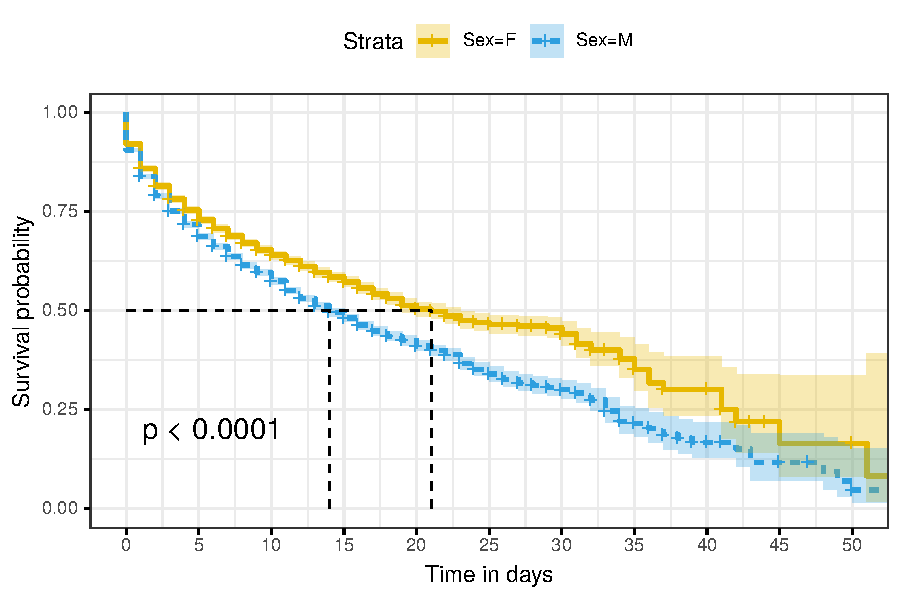
\includegraphics[width=0.97\linewidth]{sex}
		\caption{Gender stratified KM estimate}
		\label{fig:ks1}
	\end{figure}
	
	The KM estimates for gender stratification are shown in Fig: \ref{fig:ks1}. Median survival probability time  for {Male and Female is 14 and 21 days}, respectively. 
	
	\paragraph{Log Rank Test} We performed the well-known non-parametric Log Rank Test \cite{bland2004logrank} to statistically compare the difference between the survival probability of male and female strata. The  null-hypothesis of test is -- there is no difference between the two strata. 
	The test accounts for the difference in the treatment factors between the two groups. We divide the data according to the levels of the significant prognostic/treatment factors and form a stratum for each level. 
	
	For gender-based KM curve \cite{kaplan1958nonparametric} (Figure \ref{fig:ks1}) we found that $p<0.0001$, which is way less than our  $\alpha$ significance level of 5\% hence gender is statistically significant for the survival time of patients.
	
	\subsection{Age Stratified KM Estimate} To better understand the effect of age on the recovery time of patients, we stratified our patient cohort into three groups -- young (age $<18$ years old), adult (age between $18$ and $60$ years) and old (age $>$60 years).  Following the standard techniques, we computed the KM estimates for the three age strata. The same is illustrated in Fig: \ref{fig:3quant}. 
	
	\begin{figure}[h!]
		\centering
		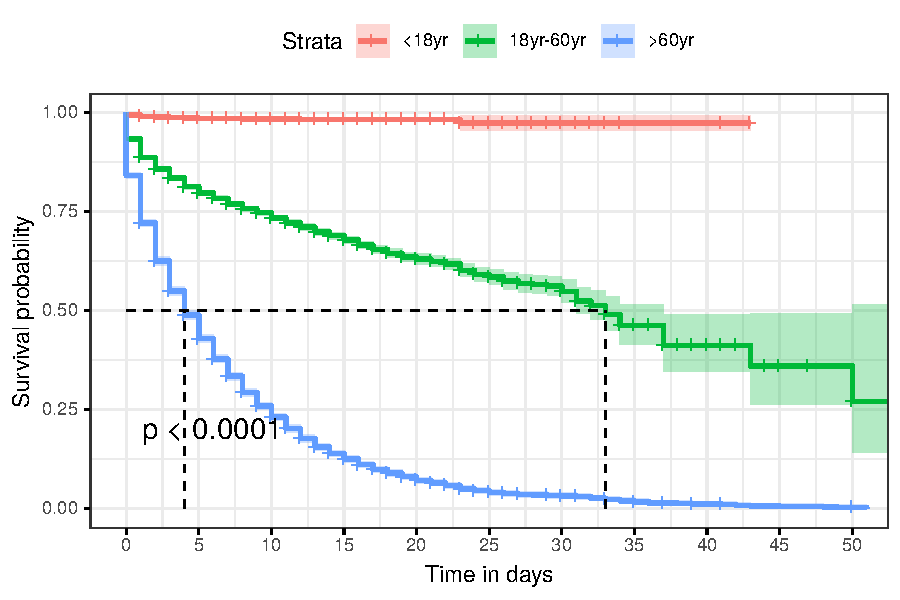
\includegraphics[width=0.97\linewidth]{3-age}
		\caption{Age stratified survival curve estimation}
		\label{fig:3quant}
	\end{figure}
	
	There was a large difference in median survival probability time  for {Adults and Old as 4 and 33 days}, respectively.  
	As expected, the \textbf{log-rank test} also validated the visual evidence with p-value $<0.0001$. 
	\section{Discussion \& Conclusion}
	
	Karnataka is one of the badly hit Indian states in terms of the number of COVID-19 cases. Further, the gender and age data was available for deceased, recovered, and active COVID-19 patients via detailed state bulletins. Hence, we performed survival analysis on the available data. Our cohort had 26,741 patients (refer Table: \ref{table:t1}). 65\% of them were male. Among all patients, 57\% of them recovered.
	Among the recovered patients, 62\% were male. The median survival time was 10 days, and the inter-quartile range (IQR) was 8 to 13 days.
	In the young cohort ($>$18 years old) of 2295 patients, 98\% of them recovered.
	Among the old cohort ($>$60 years old) of 8066 patients, mere 14\% recovered.
	In our knowledge this is largest  retrospective‐cohort based survival analysis \cite{clark2003survival} study on COVID-19 outbreak in Indian context. The data had many problems like for recovered patients co-morbidity is not recorded in the bulletins. Had this been the case, we could have fitted a Cox-proportional hazard model to assess the impact of co-morbidity in prognosis. 
	Still, this is an incremental contribution in understanding the many facets of COVID-19. 
	
	%
	%\begin{table*}[htb!]
	%	\begin{tabular}{@{}lccccccccccc@{}}
	%		\toprule
	%		\textless{}18 yr   & 2295 (100)  & 2189 (95)  & 1375 (60) & 534 (23)  & 177 (8) & 65 (3)  & 21 (1)  & 2 (0)  & 2 (0)  & 0 (0) & 0 (0) \\ 
	%		18yr -- 60 yr       & 16380 (100) & 12887 (79) & 7169 (44) & 2299 (14) & 827 (5) & 285 (2) & 130 (1) & 41 (0) & 12 (0) & 6 (0) & 4 (0) \\
	%		\textgreater{}60yr & 8066 (100)  & 3900 (48)  & 1706 (21) & 560 (7)   & 224 (3) & 78 (1)  & 48 (1)  & 25 (0) & 12 (0) & 5 (0) & 2 (0) \\\midrule
	%		days               & 0           & 5          & 10        & 15        & 20      & 25      & 30      & 35     & 40     & 45    & 50    \\ \bottomrule
	%	\end{tabular}
	%	\caption{Number of People at risk }
	%\end{table*}
	%\pagebreak
	\bibliography{example_paper.bib}
	
\end{document}
